\documentclass[11pt]{article}
\usepackage[a4paper,margin=20mm]{geometry}
\usepackage[T1]{fontenc}
\usepackage{lmodern,microtype,amsmath,amssymb,mathtools,enumitem}
\usepackage{tikz}
\usetikzlibrary{arrows.meta,calc}
\usepackage[most]{tcolorbox}
\usepackage[font=small,labelfont=bf]{caption}
\usepackage[colorlinks=true,linkcolor=blue]{hyperref}
\hypersetup{pdftitle={Coherence and Dominance under General Rankings: Handout}}
\newcommand{\M}{\mathcal M}
\newcommand{\C}{\mathcal C}
\newcommand{\U}{\mathcal U}
\newcommand{\Lf}{\mathfrak L}
\newcommand{\supp}{\operatorname{supp}}
\setlist{itemsep=1pt,topsep=3pt}
\setlength{\parindent}{0pt}
\setlength{\parskip}{4pt}

\colorlet{wone}{blue!70!black}
\colorlet{wtwo}{orange!85!black}
\colorlet{wthree}{green!50!black}
\colorlet{aone}{blue!22}
\colorlet{atwo}{orange!32}
\colorlet{athree}{green!22}

\newtcolorbox{stmt}[1]{enhanced,breakable,colback=white,colframe=black!55,boxrule=0.5pt,arc=1pt,
  left=5pt,right=5pt,top=3pt,bottom=3pt,fonttitle=\bfseries\small,coltitle=black,colbacktitle=black!8,title={#1}}
\DeclareRobustCommand{\stp}[1]{\tikz[baseline=(n.base)]\node[circle,draw,inner sep=0.7pt,minimum size=11pt,font=\scriptsize\bfseries](n){#1};}
\newenvironment{steps}{\begin{enumerate}[label=\stp{\arabic*},leftmargin=*,itemsep=2pt]}{\end{enumerate}}

\title{Coherence and Dominance under General Rankings\\[2pt]\large Handout}
\author{Jason Konek}
\date{October 2026}

\begin{document}
\maketitle

Numbering follows the paper. Two-world pictures use a ranking given by a loss: $m\preceq_\omega m'$ iff $L(m,\omega)\le L(m',\omega)$, and a model $m$ is drawn at $(L(m,1),L(m,2))$. Circled numbers in figures refer to proof steps.

\section{Setting}

\begin{stmt}{Definitions 1.1--1.4}
\begin{itemize}[leftmargin=*]
\item Worlds $\Omega\ne\varnothing$; models $\M\ne\varnothing$. A \emph{ranking} $L$: a nonempty $\M_L\subseteq\M$ (the \emph{evaluable} models) and a binary relation $\preceq_\omega$ on $\M_L$ for each $\omega\in\Omega$. No property of the relations is assumed. $L$ is \emph{transitive} if every $\preceq_\omega$ is.
\item $c$ \emph{weakly dominates} $m$: $c\preceq_\omega m$ for every $\omega$. \emph{Tied at every world}: each weakly dominates the other. $c$ \emph{dominates} $m$: $c$ weakly dominates $m$ and they are not tied at every world. $\U_L$: the undominated models.
\item $\Delta_F$: pmfs $p=(p_\omega)_{\omega\in F}$ on a finite nonempty $F\subseteq\Omega$; $\supp p=\{\omega:p_\omega>0\}$; $\delta_\omega$ the point mass at $\omega$; $\Delta\coloneqq\Delta_\Omega$ when $\Omega$ is finite.
\item Coherent models $\C\subseteq\M$, fixed in advance. $\C_L\coloneqq\C\cap\U_L$.
\end{itemize}
\end{stmt}

\begin{figure}[ht]
\centering
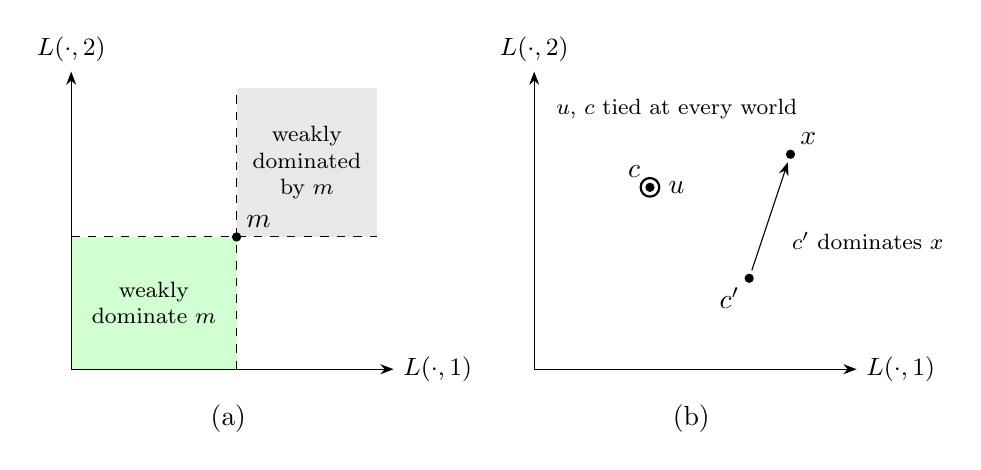
\begin{tikzpicture}[scale=1.05,>=Stealth]
\begin{scope}
 \fill[green!18] (0,0) rectangle (2,1.6);
 \fill[gray!18] (2,1.6) rectangle (3.7,3.4);
 \draw[->] (0,0) -- (3.9,0) node[right] {\small $L(\cdot,1)$};
 \draw[->] (0,0) -- (0,3.6) node[above] {\small $L(\cdot,2)$};
 \draw[dashed] (2,0) -- (2,3.4) (0,1.6) -- (3.7,1.6);
 \fill (2,1.6) circle (1.6pt) node[above right] {$m$};
 \node[align=center,font=\footnotesize] at (1,0.8) {weakly\\dominate $m$};
 \node[align=center,font=\footnotesize] at (2.85,2.5) {weakly\\dominated\\by $m$};
 \node at (1.9,-0.6) {(a)};
\end{scope}
\begin{scope}[xshift=5.6cm]
 \draw[->] (0,0) -- (3.9,0) node[right] {\small $L(\cdot,1)$};
 \draw[->] (0,0) -- (0,3.6) node[above] {\small $L(\cdot,2)$};
 \fill (1.4,2.2) circle (1.6pt) node[above left] {$c$};
 \draw[thick] (1.4,2.2) circle (3.2pt) node[right=3pt] {$u$};
 \fill (2.6,1.1) circle (1.6pt) node[below left] {$c'$};
 \fill (3.1,2.6) circle (1.6pt) node[above right] {$x$};
 \draw[->,shorten >=3pt,shorten <=3pt] (2.6,1.1) -- (3.1,2.6);
 \node[font=\footnotesize,align=left,anchor=west] at (3.0,1.55) {$c'$ dominates $x$};
 \node[font=\footnotesize,align=left,anchor=west] at (0.15,3.15) {$u$, $c$ tied at every world};
 \node at (1.9,-0.6) {(b)};
\end{scope}
\end{tikzpicture}
\caption{(a) Weak dominance. (b) Ties and dominance.}
\end{figure}

\begin{figure}[ht]
\centering
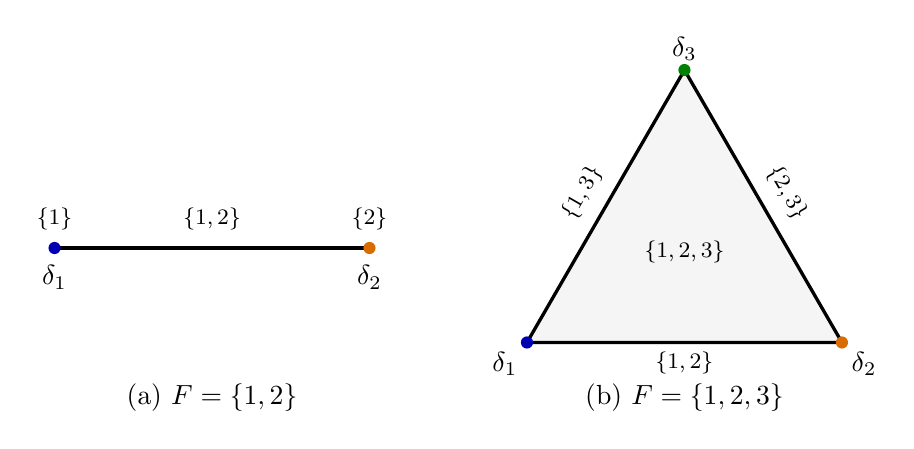
\begin{tikzpicture}[>=Stealth]
\begin{scope}[yshift=1.2cm]
 \draw[very thick] (0,0) -- (4,0);
 \fill[wone] (0,0) circle (2.2pt); \fill[wtwo] (4,0) circle (2.2pt);
 \node[below] at (0,-0.1) {$\delta_1$}; \node[below] at (4,-0.1) {$\delta_2$};
 \node[above,font=\footnotesize] at (0,0.1) {$\{1\}$};
 \node[above,font=\footnotesize] at (4,0.1) {$\{2\}$};
 \node[above,font=\footnotesize] at (2,0.1) {$\{1,2\}$};
 \node at (2,-1.9) {(a) $F=\{1,2\}$};
\end{scope}
\begin{scope}[xshift=6cm]
 \coordinate (d1) at (0,0); \coordinate (d2) at (4,0); \coordinate (d3) at (2,3.46);
 \fill[gray!8] (d1)--(d2)--(d3)--cycle;
 \draw[very thick] (d1)--(d2)--(d3)--cycle;
 \fill[wone] (d1) circle (2.2pt); \fill[wtwo] (d2) circle (2.2pt); \fill[wthree] (d3) circle (2.2pt);
 \node[below left] at (d1) {$\delta_1$}; \node[below right] at (d2) {$\delta_2$}; \node[above] at (d3) {$\delta_3$};
 \node[below,font=\footnotesize] at (2,0) {$\{1,2\}$};
 \node[font=\footnotesize,rotate=60] at (0.7,1.9) {$\{1,3\}$};
 \node[font=\footnotesize,rotate=-60] at (3.3,1.9) {$\{2,3\}$};
 \node[font=\footnotesize] at (2,1.15) {$\{1,2,3\}$};
 \node at (2,-0.7) {(b) $F=\{1,2,3\}$};
\end{scope}
\end{tikzpicture}
\caption{$\Delta_F$, with $\supp p$ marked on each face.}
\end{figure}

\subsection*{Axioms}
\begin{stmt}{Definitions 1.5--1.6}
\begin{itemize}[leftmargin=*]
\item $L$ is \emph{closed under ties}: every model tied at every world with a member of $\C_L$ is in $\C_L$.
\item For a family $\Lf$ of rankings. \emph{Evaluability}: every model in $\M$ is evaluable by some $L\in\Lf$. \emph{Coherent admissibility}: every coherent model is in $\C_L$ for some $L\in\Lf$.
\end{itemize}
\end{stmt}

\begin{stmt}{Lemma 1.7}
Let $c\in\C_L$ weakly dominate $m$. (a) If $m$ is undominated, $m$ and $c$ are tied at every world. (b) If $L$ is closed under ties and $m\notin\C_L$, then $c$ dominates $m$.
\end{stmt}
\begin{steps}
\item (a) Otherwise $c$ dominates $m$.
\item (b) Closure under ties: $m$ is not tied with $c$. So $m$ does not weakly dominate $c$, and $c$ dominates $m$.
\end{steps}

\section{The dominance theorems}

\begin{stmt}{Lemma 2.1}
Let $F$ be finite and nonempty, and let $(A_\omega)_{\omega\in F}$ be closed subsets of $\Delta_F$ such that every $p\in\Delta_F$ lies in $A_\omega$ for some $\omega\in\supp p$. Then $\bigcap_{\omega\in F}A_\omega\ne\varnothing$.
\end{stmt}

\begin{figure}[ht]
\centering
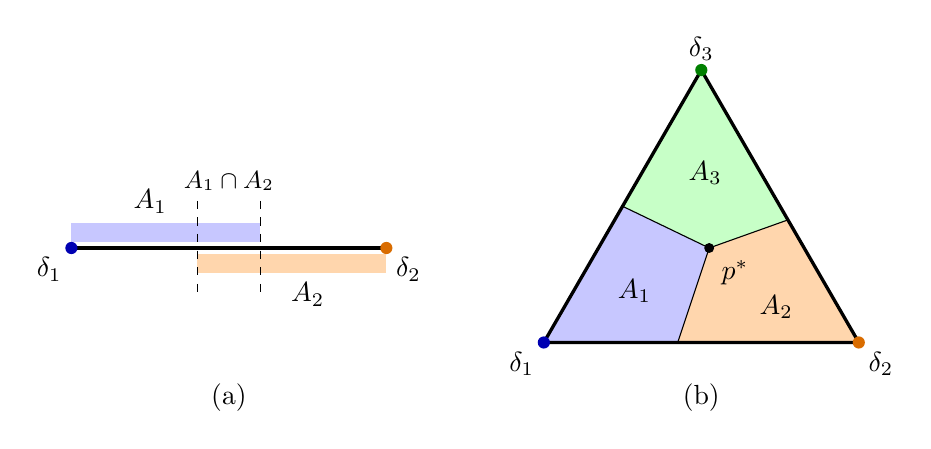
\begin{tikzpicture}
\begin{scope}[yshift=1.2cm]
 \fill[aone] (0,0.08) rectangle (2.4,0.32);
 \fill[atwo] (1.6,-0.32) rectangle (4,-0.08);
 \draw[very thick] (0,0) -- (4,0);
 \fill[wone] (0,0) circle (2.2pt); \fill[wtwo] (4,0) circle (2.2pt);
 \node[below left] at (0,0) {$\delta_1$};
 \node[below right] at (4,0) {$\delta_2$};
 \node[above] at (1.0,0.32) {$A_1$};
 \node[below] at (3.0,-0.32) {$A_2$};
 \draw[dashed] (1.6,0.6) -- (1.6,-0.6);
 \draw[dashed] (2.4,0.6) -- (2.4,-0.6);
 \node[above] at (2,0.6) {\small $A_1\cap A_2$};
 \node at (2,-1.9) {(a)};
\end{scope}
\begin{scope}[xshift=6cm]
 \coordinate (d1) at (0,0); \coordinate (d2) at (4,0); \coordinate (d3) at (2,3.46);
 \coordinate (e12) at (1.7,0); \coordinate (e23) at (3.1,1.557); \coordinate (e13) at (1,1.73);
 \coordinate (c) at (2.1,1.2);
 \fill[aone] (d1)--(e12)--(c)--(e13)--cycle;
 \fill[atwo] (d2)--(e23)--(c)--(e12)--cycle;
 \fill[athree] (d3)--(e13)--(c)--(e23)--cycle;
 \draw[very thick] (d1)--(d2)--(d3)--cycle;
 \draw (e12)--(c) (e23)--(c) (e13)--(c);
 \fill[wone] (d1) circle (2.2pt); \fill[wtwo] (d2) circle (2.2pt); \fill[wthree] (d3) circle (2.2pt);
 \node[below left] at (d1) {$\delta_1$};
 \node[below right] at (d2) {$\delta_2$};
 \node[above] at (d3) {$\delta_3$};
 \node at (1.15,0.65) {$A_1$};
 \node at (2.95,0.45) {$A_2$};
 \node at (2.05,2.15) {$A_3$};
 \fill (c) circle (1.8pt) node[below right=1pt] {$p^*$};
 \node at (2,-0.7) {(b)};
\end{scope}
\end{tikzpicture}
\caption{The hypothesis of Lemma 2.1: $\delta_\omega\in A_\omega$; each face is covered by the sets indexed by its vertices. (a) $|F|=2$. (b) $|F|=3$.}
\label{fig:kkm}
\end{figure}

\begin{figure}[ht]
\centering
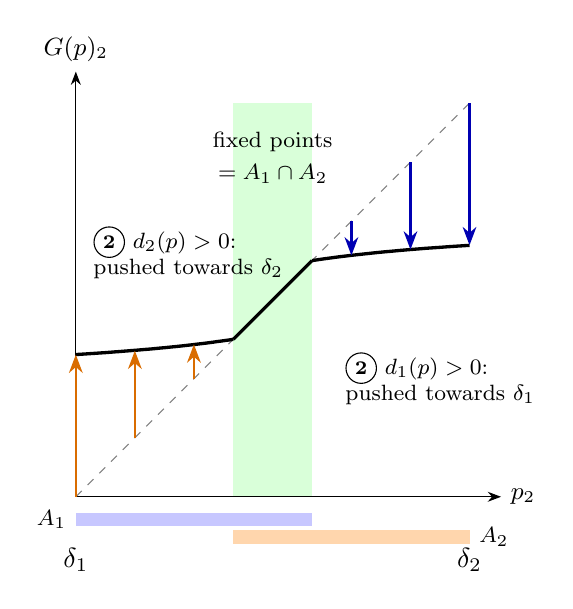
\begin{tikzpicture}[x=5cm,y=5cm,>=Stealth]
 \fill[green!15] (0.4,0) rectangle (0.6,1);
 \draw[->] (0,0) -- (1.08,0) node[right] {\small $p_2$};
 \draw[->] (0,0) -- (0,1.08) node[above] {\small $G(p)_2$};
 \draw[gray,dashed] (0,0) -- (1,1);
 \draw[very thick,black,domain=0:0.4,samples=40] plot (\x,{(\x+1.41421*(0.4-\x))/(1+1.41421*(0.4-\x))});
 \draw[very thick,black] (0.4,0.4) -- (0.6,0.6);
 \draw[very thick,black,domain=0.6:1,samples=40] plot (\x,{\x/(1+1.41421*(\x-0.6))});
 \fill[aone] (0,-0.075) rectangle (0.6,-0.04);
 \fill[atwo] (0.4,-0.12) rectangle (1,-0.085);
 \node[left,font=\footnotesize] at (0,-0.057) {$A_1$};
 \node[right,font=\footnotesize] at (1,-0.102) {$A_2$};
 \foreach \t/\g in {0.0/0.361,0.15/0.371,0.3/0.387} {\draw[->,wtwo,thick] (\t,\t) -- (\t,\g);}
 \foreach \t/\g in {0.7/0.613,0.85/0.628,1.0/0.639} {\draw[->,wone,thick] (\t,\t) -- (\t,\g);}
 \node[font=\footnotesize] at (0.5,0.9) {fixed points};
 \node[font=\footnotesize,align=center] at (0.5,0.82) {$=A_1\cap A_2$};
 \node at (0,-0.16) {$\delta_1$}; \node at (1,-0.16) {$\delta_2$};
 \node[font=\footnotesize,align=left,anchor=west] at (0.66,0.3) {\stp{2} $d_1(p)>0$:\\ pushed towards $\delta_1$};
 \node[font=\footnotesize,align=left,anchor=west] at (0.02,0.62) {\stp{2} $d_2(p)>0$:\\ pushed towards $\delta_2$};
\end{tikzpicture}
\caption{The map $G$ on $\Delta_{\{1,2\}}$, with $A_1=\{p_2\le0.6\}$ and $A_2=\{p_2\ge0.4\}$. Black: $p_2\mapsto G(p)_2$; dashed: the diagonal.}
\label{fig:brouwer}
\end{figure}

\textbf{Proof of Lemma 2.1.}
\begin{steps}
\item $\delta_\omega\in A_\omega$, since $\supp\delta_\omega=\{\omega\}$. So each $A_\omega\ne\varnothing$.
\item $d_\omega(p)\coloneqq\min_{q\in A_\omega}\lVert p-q\rVert$, $s(p)\coloneqq\sum_{\omega\in F}d_\omega(p)$, $G(p)_\omega\coloneqq(p_\omega+d_\omega(p))/(1+s(p))$. $G:\Delta_F\to\Delta_F$ is continuous.
\item Brouwer: $G(p)=p$ for some $p$; equivalently $p_\omega\, s(p)=d_\omega(p)$ for all $\omega\in F$.
\item Pick $\omega\in\supp p$ with $p\in A_\omega$: $d_\omega(p)=0$ and $p_\omega>0$, so $s(p)=0$, so $p\in\bigcap_{\omega\in F}A_\omega$.
\end{steps}

\subsection*{Finitely many worlds}
\begin{stmt}{Theorem 2.2}
Let $\Omega$ be finite and $L$ any ranking. Suppose that for each $p\in\Delta$ there is an assigned model $c_p\in\C_L$, and for each model $m$ and world $\omega$ there is a closed set $A_\omega(m)\subseteq\Delta$, such that:
\begin{enumerate}[label=(\roman*)]
\item $c_p\preceq_\omega m$ for every $p\in A_\omega(m)$;
\item for every model $m$ and every $p\in\Delta$, there is some $\omega\in\supp p$ such that $p\in A_\omega(m)$.
\end{enumerate}
Then: (a) for each model $m$, some pmf lies in every $A_\omega(m)$, and the model assigned to any such pmf weakly dominates $m$; (b) every undominated model is tied at every world with a member of $\C_L$; (c) if $L$ is closed under ties, then $\U_L=\C_L$, and every other model is dominated by a member of $\C_L$.
\end{stmt}

\begin{figure}[ht]
\centering
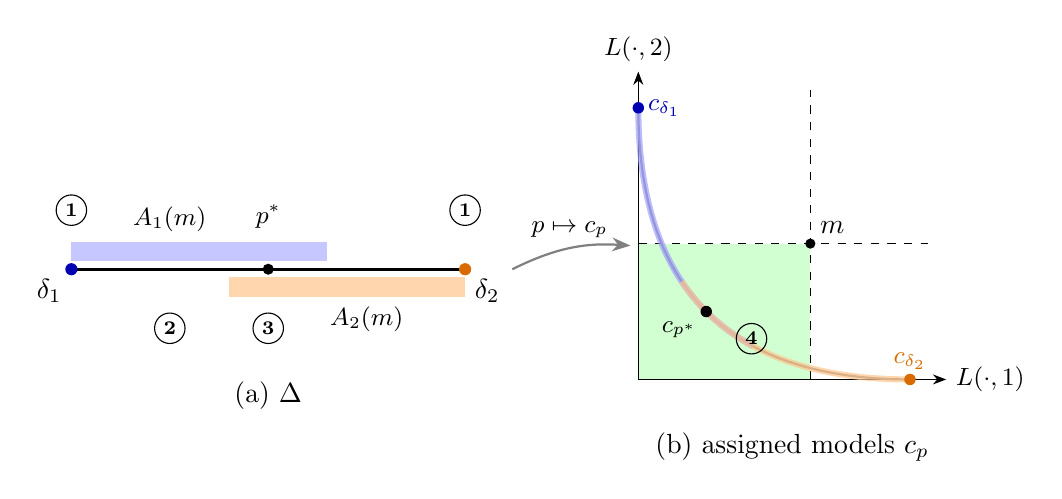
\begin{tikzpicture}[>=Stealth]
\begin{scope}[x=5cm,y=1cm]
 \fill[aone] (0,0.1) rectangle (0.65,0.35);
 \fill[atwo] (0.4,-0.35) rectangle (1,-0.1);
 \draw[very thick] (0,0) -- (1,0);
 \fill[wone] (0,0) circle (2.2pt); \fill[wtwo] (1,0) circle (2.2pt);
 \node[below left] at (0,0) {$\delta_1$}; \node[below right] at (1,0) {$\delta_2$};
 \node[above,font=\small] at (0.25,0.35) {$A_1(m)$};
 \node[below,font=\small] at (0.75,-0.35) {$A_2(m)$};
 \fill (0.5,0) circle (2pt);
 \node[above,font=\small] at (0.5,0.4) {$p^*$};
 \node at (0,0.75) {\stp{1}}; \node at (1,0.75) {\stp{1}};
 \node at (0.25,-0.75) {\stp{2}};
 \node at (0.5,-0.75) {\stp{3}};
 \node at (0.5,-1.6) {(a) $\Delta$};
\end{scope}
\begin{scope}[xshift=7.2cm,yshift=-1.4cm,scale=1.15]
 \fill[green!18] (0,0) rectangle (1.9,1.5);
 \draw[->] (0,0) -- (3.4,0) node[right] {\small $L(\cdot,1)$};
 \draw[->] (0,0) -- (0,3.4) node[above] {\small $L(\cdot,2)$};
 \draw[dashed] (1.9,0) -- (1.9,3.2);
 \draw[dashed] (0,1.5) -- (3.2,1.5);
 \draw[thick,gray,domain=0:1,samples=60] plot ({3*\x^2},{3*(1-\x)^2});
 \draw[line width=2.2pt,aone!80!blue,domain=0:0.65,samples=40,opacity=0.7] plot ({3*\x^2},{3*(1-\x)^2});
 \draw[line width=2.2pt,atwo!80!orange,domain=0.4:1,samples=40,opacity=0.7] plot ({3*\x^2},{3*(1-\x)^2});
 \fill[wone] (0,3) circle (1.8pt) node[right] {\small $c_{\delta_1}$};
 \fill[wtwo] (3,0) circle (1.8pt) node[above] {\small $c_{\delta_2}$};
 \fill (1.9,1.5) circle (1.6pt) node[above right] {$m$};
 \fill (0.75,0.75) circle (1.8pt) node[below left] {\small $c_{p^*}$};
 \node at (1.25,0.45) {\stp{4}};
 \node at (1.7,-0.75) {(b) assigned models $c_p$};
\end{scope}
\draw[->,thick,gray] (5.6,0) to[bend left=15] node[above,font=\small,black] {$p\mapsto c_p$} (7.1,0.3);
\end{tikzpicture}
\caption{Theorem 2.2(a) with two worlds and a fixed rival $m$. (a) Closed sets $A_1(m)$, $A_2(m)$. (b) Grey curve: the assigned models. Blue: $c_p$ for $p\in A_1(m)$, all at least as good as $m$ at world~1 (left of the vertical line). Orange: $c_p$ for $p\in A_2(m)$, all at least as good as $m$ at world~2 (below the horizontal line). Green: models that weakly dominate $m$.}
\label{fig:finite}
\end{figure}

\textbf{Proof.}
\begin{steps}
\item (ii) at a vertex: $\delta_\omega\in A_\omega(m)$.
\item (ii) at every $p$: the sets $A_\omega(m)$ satisfy the hypothesis of Lemma 2.1.
\item Lemma 2.1: some $p^*\in\bigcap_\omega A_\omega(m)$.
\item (i): $c_{p^*}\preceq_\omega m$ for every $\omega$. This is (a).
\item Let $m$ be any model and $c\in\C_L$ weakly dominate it. If $m$ is undominated, Lemma 1.7(a) ties $m$ to $c$: this is (b). Under closure under ties, $m\in\C_L$, so $\U_L=\C_L$; and if $m\notin\C_L$, Lemma 1.7(b) gives that $c$ dominates $m$: this is (c).
\end{steps}

\begin{stmt}{Corollary 2.3}
Let $\Omega$ be finite. Suppose that for each $p\in\Delta$ there is an assigned model $c_p\in\C_L$ such that every model $m$ has some $\omega\in\supp p$ with $c_p\preceq_\omega m$, and that each set $\{p:c_p\preceq_\omega m\}$ is closed. Then the conclusions of Theorem 2.2 hold.
\end{stmt}
\begin{steps}
\item $A_\omega(m)\coloneqq\{p:c_p\preceq_\omega m\}$. In Figure~\ref{fig:finite}: $A_1(m)$ is the set of all $p$ whose $c_p$ lies left of the vertical line, $A_2(m)$ the set of all $p$ whose $c_p$ lies below the horizontal line.
\end{steps}

\subsection*{Arbitrary sets of worlds}
\begin{stmt}{Theorem 2.4}
Let $\Omega$ be any nonempty set and $L$ any ranking. Suppose:
\begin{enumerate}[label=\arabic*.,leftmargin=*]
\item There is a compact space of parameters $\Theta$. For each $\theta\in\Theta$, there is a selected model $c_\theta\in\C_L$. For each world $\omega$ and model $m$ there is a closed set $K_\omega(m)\subseteq\Theta$ such that $c_\theta\preceq_\omega m$ for every $\theta\in K_\omega(m)$.
\item For every finite set of worlds $G\subseteq\Omega$, there are a nonempty finite set $F\supseteq G$, a map $\theta_F:\Delta_F\to\Theta$, and, for each $\omega\in F$ and model $m$, a closed set $A^F_\omega(m)\subseteq\Delta_F$, such that
\begin{enumerate}[label=(\alph*)]
\item for every $\omega\in F$ and model $m$, $\theta_F(p)\in K_\omega(m)$ for all $p\in A^F_\omega(m)$;
\item for every model $m$ and every $p\in\Delta_F$, there is some $\omega\in\supp p$ such that $p\in A^F_\omega(m)$.
\end{enumerate}
\end{enumerate}
Then every model is weakly dominated by some $c_\theta$, and conclusions (b) and (c) of Theorem 2.2 hold.
\end{stmt}

\begin{figure}[ht]
\centering
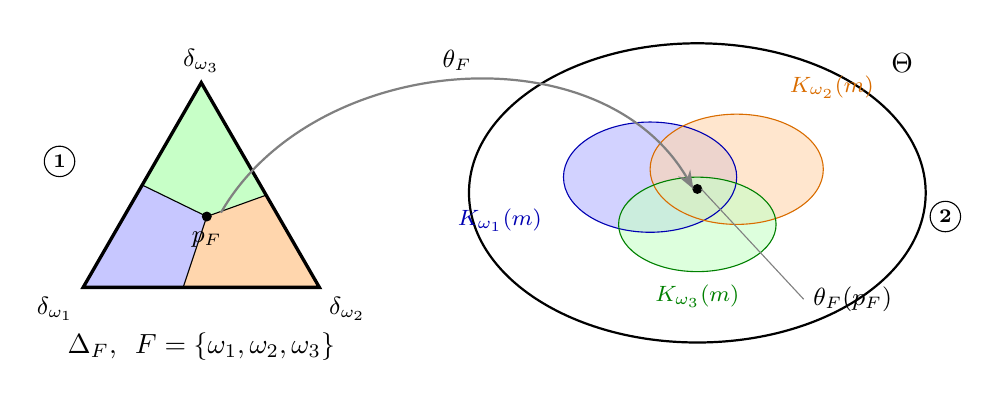
\begin{tikzpicture}[>=Stealth]
\begin{scope}
 \coordinate (d1) at (0,0); \coordinate (d2) at (3,0); \coordinate (d3) at (1.5,2.6);
 \coordinate (e12) at (1.27,0); \coordinate (e23) at (2.32,1.17); \coordinate (e13) at (0.75,1.3);
 \coordinate (c) at (1.57,0.9);
 \fill[aone] (d1)--(e12)--(c)--(e13)--cycle;
 \fill[atwo] (d2)--(e23)--(c)--(e12)--cycle;
 \fill[athree] (d3)--(e13)--(c)--(e23)--cycle;
 \draw[very thick] (d1)--(d2)--(d3)--cycle;
 \draw (e12)--(c) (e23)--(c) (e13)--(c);
 \node[below left,font=\small] at (d1) {$\delta_{\omega_1}$};
 \node[below right,font=\small] at (d2) {$\delta_{\omega_2}$};
 \node[above,font=\small] at (d3) {$\delta_{\omega_3}$};
 \fill (c) circle (1.8pt) node[below=2pt,font=\small] {$p_F$};
 \node at (-0.3,1.6) {\stp{1}};
 \node at (1.5,-0.75) {$\Delta_F$, \ $F=\{\omega_1,\omega_2,\omega_3\}$};
\end{scope}
\begin{scope}[xshift=7.8cm,yshift=1.2cm]
 \draw[thick] (0,0) ellipse (2.9 and 1.9);
 \node at (2.6,1.65) {$\Theta$};
 \fill[aone,opacity=0.8] (-0.6,0.2) ellipse (1.1 and 0.7);
 \fill[atwo,opacity=0.6] (0.5,0.3) ellipse (1.1 and 0.7);
 \fill[athree,opacity=0.6] (0,-0.4) ellipse (1.0 and 0.6);
 \draw[wone] (-0.6,0.2) ellipse (1.1 and 0.7);
 \draw[wtwo] (0.5,0.3) ellipse (1.1 and 0.7);
 \draw[wthree] (0,-0.4) ellipse (1.0 and 0.6);
 \node[font=\footnotesize,wone,anchor=east] at (-1.85,-0.35) {$K_{\omega_1}(m)$};
 \node[font=\footnotesize,wtwo,anchor=south west] at (1.05,1.08) {$K_{\omega_2}(m)$};
 \node[font=\footnotesize,wthree,anchor=north] at (0,-1.05) {$K_{\omega_3}(m)$};
 \fill (0,0.05) circle (1.8pt);
 \draw[gray] (0.05,0.05) -- (1.35,-1.35) node[right,black,font=\small] {$\theta_F(p_F)$};
 \node at (3.15,-0.3) {\stp{2}};
\end{scope}
\draw[->,thick,gray] (1.75,0.95) to[out=60,in=120] node[above,font=\small,black] {$\theta_F$} (7.75,1.25);
\end{tikzpicture}
\caption{One finite $F$. Lemma 2.1 on $\Delta_F$ gives $p_F$; assumption 2(a) sends it into $\bigcap_{\omega\in F}K_\omega(m)$.}
\label{fig:local-a}
\end{figure}

\begin{figure}[ht]
\centering
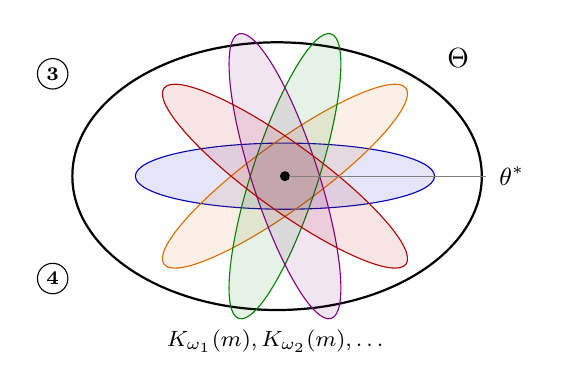
\begin{tikzpicture}[>=Stealth]
\begin{scope}
 \draw[thick] (0,0) ellipse (2.6 and 1.7);
 \node at (2.3,1.5) {$\Theta$};
 \foreach \a/\col in {0/wone,36/wtwo,72/wthree,108/violet,144/red!70!black} {
   \fill[\col,opacity=0.10,rotate around={\a:(0.1,0)}] (0.1,0) ellipse (1.9 and 0.42);
   \draw[\col,rotate around={\a:(0.1,0)}] (0.1,0) ellipse (1.9 and 0.42);
 }
 \fill (0.1,0) circle (1.8pt);
 \node[font=\small,anchor=west] at (2.7,0) {$\theta^*$};
 \draw[gray] (0.15,0) -- (2.65,0);
 \node[font=\footnotesize,align=center] at (0,-2.1) {$K_{\omega_1}(m),K_{\omega_2}(m),\dots$};
 \node at (-2.85,1.3) {\stp{3}};
 \node at (-2.85,-1.3) {\stp{4}};
\end{scope}
\end{tikzpicture}
\caption{Every finite subfamily of the closed sets $K_\omega(m)$, $\omega\in\Omega$, has a nonempty intersection; compactness gives $\theta^*$ in all of them.}
\label{fig:local-b}
\end{figure}

\textbf{Proof.} Fix a model $m$.
\begin{steps}
\item For any $F$ from assumption 2, the sets $A^F_\omega(m)$, $\omega\in F$, satisfy the hypothesis of Lemma 2.1, by 2(b). So some $p_F\in\bigcap_{\omega\in F}A^F_\omega(m)$.
\item By 2(a), $\theta_F(p_F)\in\bigcap_{\omega\in F}K_\omega(m)$.
\item Given $\omega_1,\dots,\omega_k$, apply assumption 2 to $G=\{\omega_1,\dots,\omega_k\}$: $\bigcap_iK_{\omega_i}(m)\supseteq\bigcap_{\omega\in F}K_\omega(m)\ni\theta_F(p_F)$. Every finite subfamily of the closed sets $K_\omega(m)$ has a nonempty intersection.
\item If $\bigcap_{\omega\in\Omega}K_\omega(m)=\varnothing$, the open sets $\Theta\setminus K_\omega(m)$ cover $\Theta$. By compactness, finitely many, $\Theta\setminus K_{\omega_1}(m),\dots,\Theta\setminus K_{\omega_k}(m)$, cover $\Theta$, so $\bigcap_iK_{\omega_i}(m)=\varnothing$, contradicting step 3. So some $\theta^*\in\bigcap_{\omega\in\Omega}K_\omega(m)$.
\item By assumption 1, $c_{\theta^*}\preceq_\omega m$ for every $\omega$. Conclusions (b) and (c): step 5 of the proof of Theorem 2.2.
\end{steps}

\section{The dominance argument}

\begin{stmt}{Propositions 3.1 and 3.2}
Let $L$ be a ranking under which every model is weakly dominated by a member of $\C_L$.
\begin{itemize}[leftmargin=*]
\item[3.1] Every undominated model is tied at every world with a member of $\C_L$. If $L$ is also closed under ties, then $\U_L=\C_L$, and every other model is dominated by a member of $\C_L$.
\item[3.2] If $L$ is transitive, then $\U_L$ consists of the models tied at every world with some member of $\C_L$, and every other model is dominated by a member of $\C_L$.
\end{itemize}
\end{stmt}

\begin{figure}[ht]
\centering
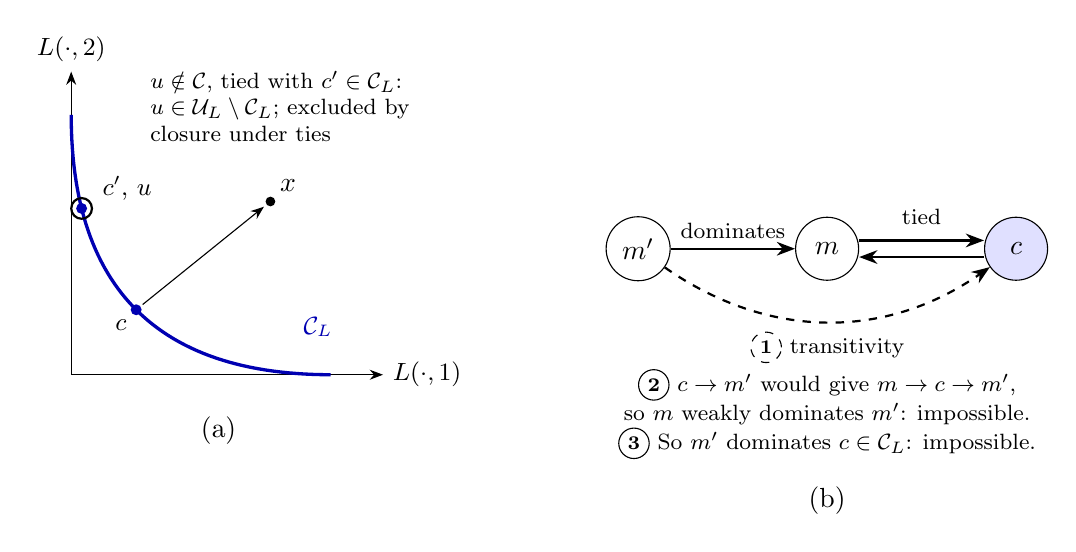
\begin{tikzpicture}[>=Stealth]
\begin{scope}[scale=1.1]
 \draw[->] (0,0) -- (3.6,0) node[right] {\small $L(\cdot,1)$};
 \draw[->] (0,0) -- (0,3.5) node[above] {\small $L(\cdot,2)$};
 \draw[very thick,wone,domain=0:1,samples=60] plot ({3*\x^2},{3*(1-\x)^2});
 \node[wone,font=\small] at (2.85,0.55) {$\C_L$};
 \fill[wone] (0.75,0.75) circle (1.8pt) node[below left,black] {\small $c$};
 \fill (2.3,2.0) circle (1.6pt) node[above right] {$x$};
 \draw[->,shorten >=3pt,shorten <=3pt] (0.75,0.75) -- (2.3,2.0);
 \fill[wone] (0.12,1.92) circle (1.8pt);
 \draw[thick] (0.12,1.92) circle (3.4pt);
 \node[font=\small,anchor=west] at (0.25,2.15) {$c'$, $u$};
 \node[font=\footnotesize,align=left,anchor=west] at (0.8,3.1) {$u\notin\C$, tied with $c'\in\C_L$:\\ $u\in\U_L\setminus\C_L$; excluded by\\ closure under ties};
 \node at (1.7,-0.65) {(a)};
\end{scope}
\begin{scope}[xshift=7.2cm,yshift=1.6cm]
 \node[circle,draw,minimum size=0.8cm] (mp) at (0,0) {$m'$};
 \node[circle,draw,minimum size=0.8cm] (m) at (2.4,0) {$m$};
 \node[circle,draw,fill=blue!12,minimum size=0.8cm] (c) at (4.8,0) {$c$};
 \draw[->,thick] (mp) -- node[above,font=\footnotesize] {dominates} (m);
 \draw[->,thick] ([yshift=3pt]m.east) -- ([yshift=3pt]c.west);
 \draw[->,thick] ([yshift=-3pt]c.west) -- ([yshift=-3pt]m.east);
 \node[font=\footnotesize] at (3.6,0.4) {tied};
 \draw[->,thick,dashed] (mp) to[bend right=35] node[below,font=\footnotesize] {\stp{1} transitivity} (c);
 \node[font=\footnotesize,align=center] at (2.4,-2.1) {\stp{2} $c\to m'$ would give $m\to c\to m'$,\\ so $m$ weakly dominates $m'$: impossible.\\ \stp{3} So $m'$ dominates $c\in\C_L$: impossible.};
 \node at (2.4,-3.2) {(b)};
\end{scope}
\end{tikzpicture}
\caption{(a) Proposition 3.1. (b) Proposition 3.2: a model $m$ tied with $c\in\C_L$ is undominated. Arrow $a\to b$: $a\preceq_\omega b$ at every world.}
\label{fig:conclusion}
\end{figure}

\textbf{Proof of 3.1.} Lemma 1.7 applied to each model and a member of $\C_L$ weakly dominating it.

\textbf{Proof of 3.2.}
\begin{steps}
\item Let $m$ be tied with $c\in\C_L$ and $m'$ dominate $m$. Then $m'\preceq_\omega m\preceq_\omega c$, so $m'$ weakly dominates $c$.
\item If $c$ weakly dominated $m'$, then $m\preceq_\omega c\preceq_\omega m'$: $m$ weakly dominates $m'$, contradicting that $m'$ dominates $m$.
\item So $m'$ dominates $c\in\C_L$: impossible. So $m\in\U_L$. A dominated $m$ is not tied with its weak dominator $c\in\C_L$, so $c$ dominates $m$.
\end{steps}

\begin{stmt}{Definition 3.3 and Proposition 3.4}
A model is \emph{irrational} if every ranking in $\Lf$ that evaluates it has an undominated model that dominates it; \emph{rationally permissible} if it is undominated under some ranking in $\Lf$.

Suppose that under each $L\in\Lf$, every model in $\M_L$ is weakly dominated by a member of $\C_L$. Then for each $L\in\Lf$: (a) every undominated model is tied at every world with a member of $\C_L$; (b) if $L$ is closed under ties, then $\U_L=\C_L$, and every other model in $\M_L$ is dominated by a member of $\C_L$; (c) if $L$ is transitive, then $\U_L$ consists of the models tied at every world with a member of $\C_L$, and every other model in $\M_L$ is dominated by a member of $\C_L$.

If every ranking in $\Lf$ is closed under ties or transitive, then a model is undominated under no ranking iff, under every ranking that evaluates it, some undominated model dominates it. Coherent admissibility alone, without this assumption, makes every coherent model rationally permissible. If, in addition, every ranking in $\Lf$ is closed under ties, the rationally permissible models are exactly the coherent ones.
\end{stmt}

\begin{figure}[ht]
\centering
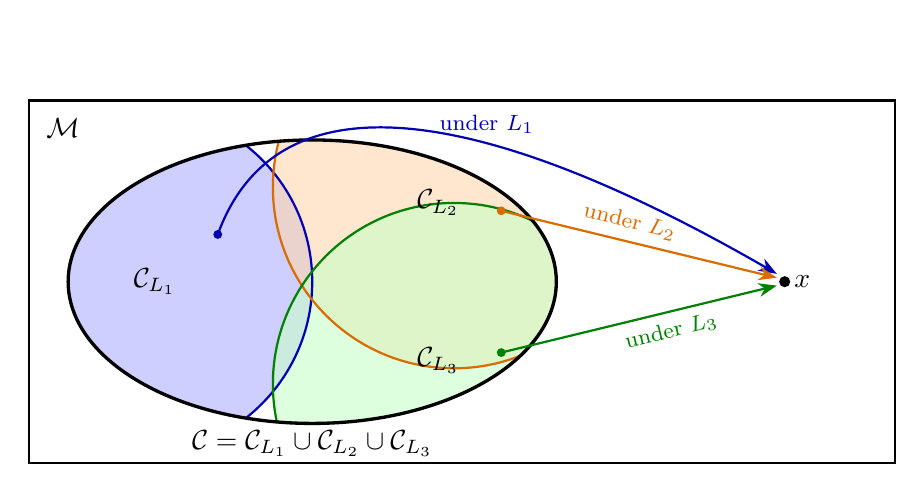
\begin{tikzpicture}[>=Stealth]
 \draw[thick] (0,0) rectangle (11,4.6);
 \node[anchor=north west] at (0.1,4.5) {$\M$};
 \begin{scope}
  \clip (3.6,2.3) ellipse (3.1 and 1.8);
  \fill[aone,opacity=0.85] (1.4,2.3) circle (2.2);
  \fill[atwo,opacity=0.6] (5.4,3.5) circle (2.3);
  \fill[athree,opacity=0.6] (5.4,1.0) circle (2.3);
  \draw[wone,thick] (1.4,2.3) circle (2.2);
  \draw[wtwo,thick] (5.4,3.5) circle (2.3);
  \draw[wthree,thick] (5.4,1.0) circle (2.3);
 \end{scope}
 \draw[very thick] (3.6,2.3) ellipse (3.1 and 1.8);
 \node at (1.6,2.3) {$\C_{L_1}$};
 \node at (5.2,3.3) {$\C_{L_2}$};
 \node at (5.2,1.3) {$\C_{L_3}$};
 \node at (3.6,0.25) {$\C=\C_{L_1}\cup\C_{L_2}\cup\C_{L_3}$};
 \fill (9.6,2.3) circle (2pt) node[right] {$x$};
 \fill[wone] (2.4,2.9) circle (1.6pt);
 \fill[wtwo] (6.0,3.2) circle (1.6pt);
 \fill[wthree] (6.0,1.4) circle (1.6pt);
 \draw[->,wone,thick] (2.4,2.9) to[out=70,in=150] node[pos=0.55,above,font=\footnotesize] {under $L_1$} (9.5,2.4);
 \draw[->,wtwo,thick] (6.0,3.2) -- node[pos=0.45,above,sloped,font=\footnotesize] {under $L_2$} (9.5,2.35);
 \draw[->,wthree,thick] (6.0,1.4) -- node[pos=0.6,below,sloped,font=\footnotesize] {under $L_3$} (9.5,2.25);
\end{tikzpicture}
\caption{Proposition 3.4 with $\Lf=\{L_1,L_2,L_3\}$, each closed under ties. Coherent admissibility: the sets $\C_{L_i}$ cover $\C$. Each $\U_{L_i}=\C_{L_i}$, so the rationally permissible models are $\bigcup_i\C_{L_i}=\C$. An incoherent $x$ is dominated by a member of $\C_{L_i}$ under each $L_i$ that evaluates it. Arrows: dominates.}
\label{fig:permissible}
\end{figure}

\textbf{Proof of 3.4.}
\begin{steps}
\item (a), (b): Proposition 3.1. (c): Proposition 3.2.
\item $m\notin\bigcup_L\U_L$: under each $L$ evaluating $m$, by (b) or (c), some member of $\C_L\subseteq\U_L$ dominates $m$. Converse: from the definitions.
\item Coherent admissibility: $\C\subseteq\bigcup_L\C_L\subseteq\bigcup_L\U_L$.
\item All $L$ closed under ties: $\bigcup_L\U_L=\bigcup_L\C_L=\C$, since each $\C_L\subseteq\C$.
\end{steps}

\end{document}
